
\documentclass[11pt]{article}
% ------- TikZ Preamble -------
\RequirePackage{tikz}
\usetikzlibrary{knots,hobby,calc,arrows.meta, intersections,decorations.pathreplacing,decorations.markings,shapes.geometric,spath3}
\usepackage{amsmath}
\usepackage{hyperref}
\usepackage{calc,pict2e}
% stix replaces amssymb/amsfonts; loading both exceeds the symbol-font limit ("Too many symbol fonts declared").
\usepackage{stix}

\tikzset{
  knot diagram/every strand/.append style={
    ultra thick,
    black
  },
  show curve controls/.style={
    postaction=decorate,
    decoration={show path construction,
      curveto code={
        \draw [blue, dashed]
        (\tikzinputsegmentfirst) -- (\tikzinputsegmentsupporta)
        node [at end, draw, solid, red, inner sep=2pt]{};
        \draw [blue, dashed]
        (\tikzinputsegmentsupportb) -- (\tikzinputsegmentlast)
        node [at start, draw, solid, red, inner sep=2pt]{}
        node [at end, fill, blue, ellipse, inner sep=2pt]{}
        ;
      }
    }
  },
  show curve endpoints/.style={
    postaction=decorate,
    decoration={show path construction,
      curveto code={
        \node [fill, blue, ellipse, inner sep=2pt] at (\tikzinputsegmentlast) {}
        ;
      }
    }
  }
}



% Document
\begin{document}




% --- 3₁ Half-Twist Trefoil ---
    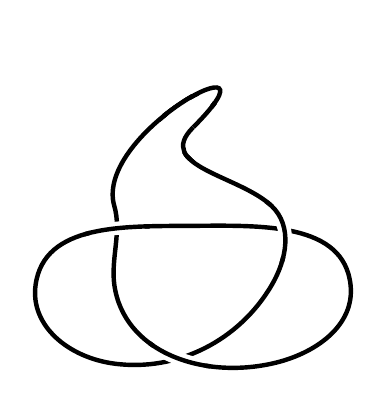
\begin{tikzpicture}[use Hobby shortcut]
    \coordinate (P1) at (0.0, 2.0);
    \coordinate (P2) at (-1.0, 1.0);
    \coordinate (P3) at (-1.0, 0.0);
    \coordinate (P4) at (1.0, -1.0);
    \coordinate (P5) at (2.0, 0.0);
    \coordinate (P6) at (0.0, 0.75);
    \coordinate (P7) at (-2.0, 0.0);
    \coordinate (P8) at (-1.0, -1.0);
    \coordinate (P9) at (1.0, 0.0);
    \coordinate (P10) at (1.0, 1.0);
    \coordinate (P11) at (0.0, 2.0);
    \coordinate (P12) at (0.0, 2.0);
    \begin{knot}[
        consider self intersections,
        ignore endpoint intersections=false,
        flip crossing/.list={2,4,6,8,10,12,14},
    ]
        \strand ([closed] P1)..(P2)..(P3)..(P4)..(P5)..(P6)..(P7)..(P8)..(P9)..(P10)..(P11)..(P12);
    \end{knot}
    \end{tikzpicture}

% --- 4₁ Two-Half-Twist ---
    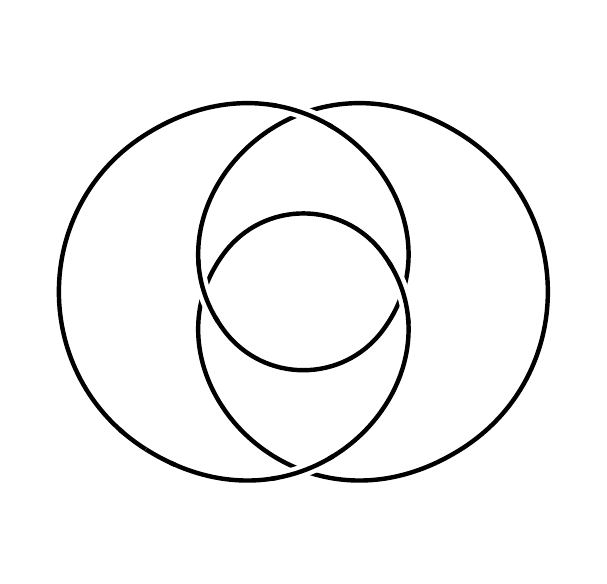
\begin{tikzpicture}[use Hobby shortcut]
    \coordinate (P1) at (-2.0, -2.0);
    \coordinate (P2) at (-2.0, 2.0);
    \coordinate (P3) at (1.0, -0.5);
    \coordinate (P4) at (-1.0, -0.5);
    \coordinate (P5) at (2.0, 2.0);
    \coordinate (P6) at (2.0, -2.0);
    \coordinate (P7) at (-1.0, 0.5);
    \coordinate (P8) at (1.0, 0.5);
    \coordinate (P9) at (-2.0, -2.0);
    \begin{knot}[
        consider self intersections,
        ignore endpoint intersections=false,
        flip crossing/.list={2,4,6,8,10,12,14},
    ]
        \strand ([closed] P1)..(P2)..(P3)..(P4)..(P5)..(P6)..(P7)..(P8)..(P9);
    \end{knot}
    \end{tikzpicture}




% --- 5₂ Three-Half-Twist ---
    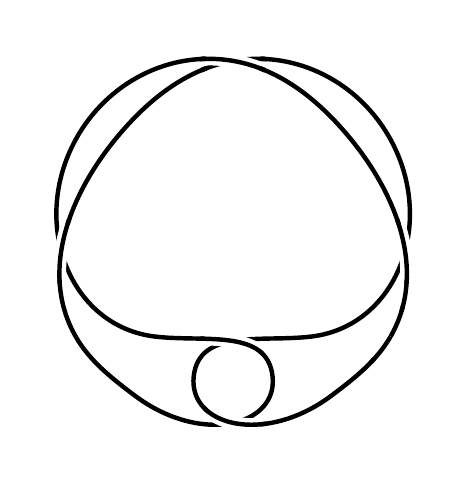
\begin{tikzpicture}[use Hobby shortcut]
    \coordinate (P1) at (2.0, -1.5);
    \coordinate (P2) at (1.5, 1.0);
    \coordinate (P3) at (0.0, 2.0);
    \coordinate (P4) at (-2.0, 1.0);
    \coordinate (P5) at (-1.0, -1.5);
    \coordinate (P6) at (0.5, -2.0);
    \coordinate (P7) at (-1.25, -2.25);
    \coordinate (P8) at (-2.0, -1.5);
    \coordinate (P9) at (-1.5, 1.0);
    \coordinate (P10) at (0.0, 2.0);
    \coordinate (P11) at (2.0, 1.0);
    \coordinate (P12) at (1.0, -1.5);
    \coordinate (P13) at (-0.5, -2.0);
    \coordinate (P14) at (1.25, -2.25);
    \coordinate (P15) at (2.0, -1.5);
    \begin{knot}[
        consider self intersections,
        ignore endpoint intersections=false,
        flip crossing/.list={2,4,6,8,10,12,14,16,18},
    ]
        \strand ([closed] P1)..(P2)..(P3)..(P4)..(P5)..(P6)..(P7)..(P8)..(P9)..(P10)..(P11)..(P12)..(P13)..(P14)..(P15);
    \end{knot}
    \end{tikzpicture}

% --- 6₁ Four-Half-Twist ---
    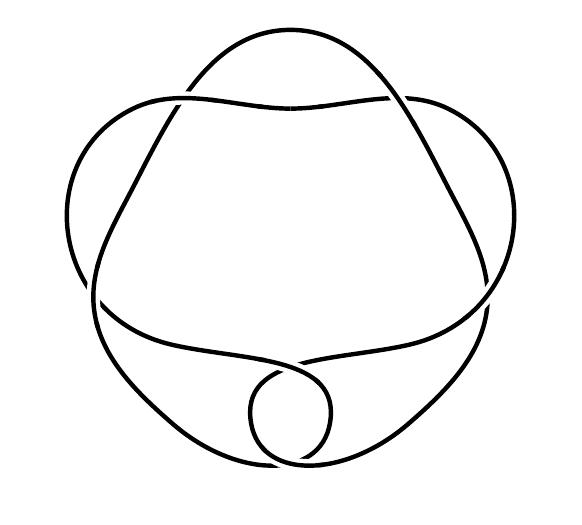
\begin{tikzpicture}[use Hobby shortcut]
    \coordinate (P1) at (0.0, 2.0);
    \coordinate (P2) at (-2.0, 2.0);
    \coordinate (P3) at (-1.5, -1.0);
    \coordinate (P4) at (0.5, -2.0);
    \coordinate (P5) at (-1.5, -2.0);
    \coordinate (P6) at (-2.5, -0.5);
    \coordinate (P7) at (-2.0, 1.0);
    \coordinate (P8) at (0.0, 3.0);
    \coordinate (P9) at (2.0, 1.0);
    \coordinate (P10) at (2.5, -0.5);
    \coordinate (P11) at (1.5, -2.0);
    \coordinate (P12) at (-0.5, -2.0);
    \coordinate (P13) at (1.5, -1.0);
    \coordinate (P14) at (2.0, 2.0);
    \coordinate (P15) at (0.0, 2.0);
    \begin{knot}[
        consider self intersections,
        ignore endpoint intersections=false,
        flip crossing/.list={2,4,6,8,10,12,14,16,18},
    ]
        \strand ([closed] P1)..(P2)..(P3)..(P4)..(P5)..(P6)..(P7)..(P8)..(P9)..(P10)..(P11)..(P12)..(P13)..(P14)..(P15);
    \end{knot}
    \end{tikzpicture}


% --- 7₂ Twist ---
    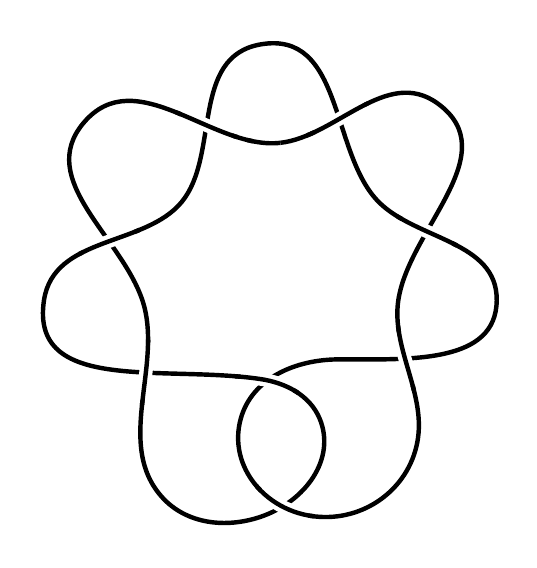
\begin{tikzpicture}[use Hobby shortcut]
    \coordinate (P1) at (0.0, 2.0);
    \coordinate (P2) at (-2.50, 2.25);
    \coordinate (P3) at (-1.75, 0.0);
    \coordinate (P4) at (-1.50, -2.50);
    \coordinate (P5) at (-0.25, -2.75);
    \coordinate (P6) at (0.50, -1.50);
    \coordinate (P7) at (-0.25, -1.0);
    \coordinate (P8) at (-3.0, 0.0);
    \coordinate (P9) at (-1.25, 1.25);
    \coordinate (P10) at (-0.25, 3.25);
    \coordinate (P11) at (1.25, 1.25);
    \coordinate (P12) at (2.75, 0.0);
    \coordinate (P13) at (0.75, -0.75);
    \coordinate (P14) at (-0.50, -1.50);
    \coordinate (P15) at (0.50, -2.75);
    \coordinate (P16) at (1.75, -1.75);
    \coordinate (P17) at (1.50, 0.0);
    \coordinate (P18) at (2.0, 2.50);
    \coordinate (P19) at (0.0, 2.0);
    \begin{knot}[
        consider self intersections,
        ignore endpoint intersections=false,
        flip crossing/.list={2,4,6,8,10,12,14,16,18,20},
    ]
        \strand ([closed] P1)..(P2)..(P3)..(P4)..(P5)..(P6)..(P7)..(P8)..(P9)..(P10)..(P11)..(P12)..(P13)..(P14)..(P15)..(P16)..(P17)..(P18)..(P19);
    \end{knot}
    \end{tikzpicture}

% --- 8₁ Twist Octafoil ---
    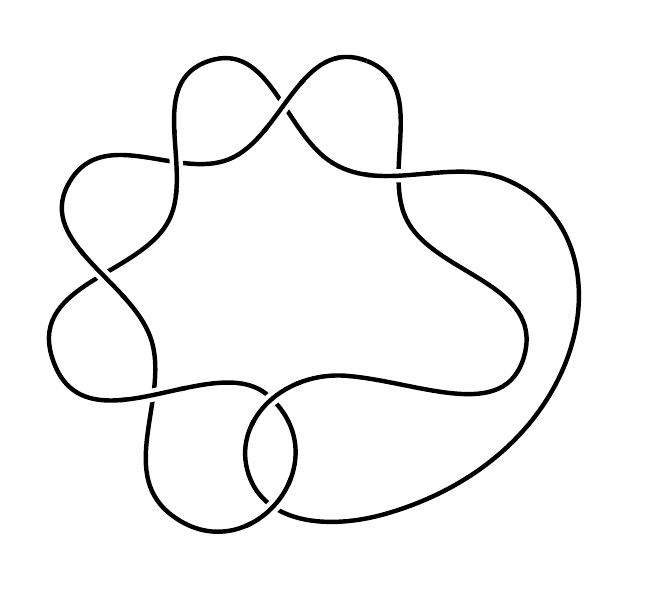
\begin{tikzpicture}[use Hobby shortcut]
    \coordinate (P1) at (0.75, 3.25);
    \coordinate (P2) at (-1.0, 2.0);
    \coordinate (P3) at (-3.0, 1.75);
    \coordinate (P4) at (-2.0, -0.25);
    \coordinate (P5) at (-1.75, -2.50);
    \coordinate (P6) at (-0.50, -1.0);
    \coordinate (P7) at (-3.25, -0.50);
    \coordinate (P8) at (-1.75, 1.25);
    \coordinate (P9) at (-1.25, 3.25);
    \coordinate (P10) at (0.25, 2.0);
    \coordinate (P11) at (2.50, 1.75);
    \coordinate (P12) at (1.0, -2.50);
    \coordinate (P13) at (-0.75, -2.0);
    \coordinate (P14) at (0.50, -0.75);
    \coordinate (P15) at (2.75, -0.50);
    \coordinate (P16) at (1.25, 1.25);
    \coordinate (P17) at (0.75, 3.25);
    \begin{knot}[
        consider self intersections,
        ignore endpoint intersections=false,
        flip crossing/.list={2,4,6,8,10,12,14,16,18,20},
    ]
        \strand ([closed] P1)..(P2)..(P3)..(P4)..(P5)..(P6)..(P7)..(P8)..(P9)..(P10)..(P11)..(P12)..(P13)..(P14)..(P15)..(P16)..(P17);
    \end{knot}
    \end{tikzpicture}


% --- 9₂ Twist ---
    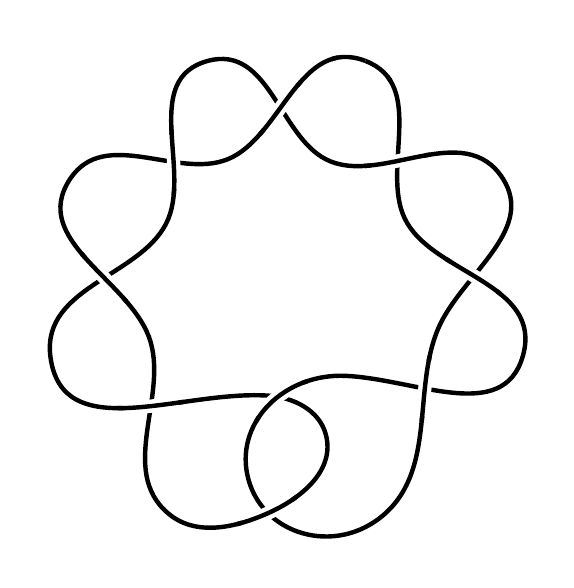
\begin{tikzpicture}[use Hobby shortcut]
    \coordinate (P1) at (0.75, 3.25);
    \coordinate (P2) at (-1.0, 2.0);
    \coordinate (P3) at (-3.0, 1.75);
    \coordinate (P4) at (-2.0, -0.25);
    \coordinate (P5) at (-1.75, -2.50);
    \coordinate (P6) at (-0.50, -2.50);
    \coordinate (P7) at (0.25, -1.50);
    \coordinate (P8) at (-0.50, -1.0);
    \coordinate (P9) at (-3.25, -0.50);
    \coordinate (P10) at (-1.75, 1.25);
    \coordinate (P11) at (-1.25, 3.25);
    \coordinate (P12) at (0.25, 2.0);
    \coordinate (P13) at (2.50, 1.75);
    \coordinate (P14) at (1.75, 0.0);
    \coordinate (P15) at (1.0, -2.50);
    \coordinate (P16) at (-0.75, -2.0);
    \coordinate (P17) at (0.50, -0.75);
    \coordinate (P18) at (2.75, -0.50);
    \coordinate (P19) at (1.25, 1.25);
    \coordinate (P20) at (0.75, 3.25);
    \begin{knot}[
        consider self intersections,
        ignore endpoint intersections=false,
        flip crossing/.list={2,4,6,8,10,12,14,16,18,20},
    ]
        \strand ([closed] P1)..(P2)..(P3)..(P4)..(P5)..(P6)..(P7)..(P8)..(P9)..(P10)..(P11)..(P12)..(P13)..(P14)..(P15)..(P16)..(P17)..(P18)..(P19)..(P20);
    \end{knot}
    \end{tikzpicture}

% --- 10₁ Twist Dekafoil ---
    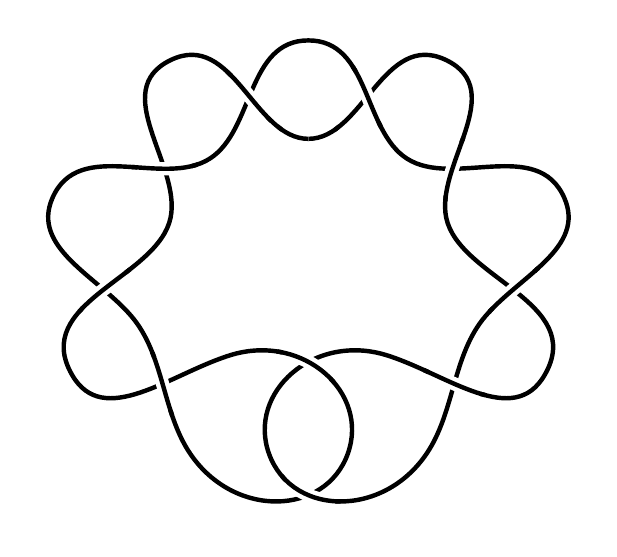
\begin{tikzpicture}[use Hobby shortcut]
    \coordinate (P1) at (0.0, 2.0);
    \coordinate (P2) at (-1.75, 3.0);
    \coordinate (P3) at (-1.75, 1.0);
    \coordinate (P4) at (-3.0, -1.0);
    \coordinate (P5) at (-1.0, -0.75);
    \coordinate (P6) at (0.50, -2.0);
    \coordinate (P7) at (-1.50, -2.0);
    \coordinate (P8) at (-2.25, -0.25);
    \coordinate (P9) at (-3.25, 1.25);
    \coordinate (P10) at (-1.25, 1.75);
    \coordinate (P11) at (0.0, 3.25);
    \coordinate (P12) at (1.25, 1.75);
    \coordinate (P13) at (3.25, 1.25);
    \coordinate (P14) at (2.25, -0.25);
    \coordinate (P15) at (1.50, -2.0);
    \coordinate (P16) at (-0.50, -2.0);
    \coordinate (P17) at (1.0, -0.75);
    \coordinate (P18) at (3.0, -1.0);
    \coordinate (P19) at (1.75, 1.0);
    \coordinate (P20) at (1.75, 3.0);
    \coordinate (P21) at (0.0, 2.0);
    \begin{knot}[
        consider self intersections,
        ignore endpoint intersections=false,
        flip crossing/.list={2,4,6,8,10,12,14,16,18,20},
    ]
        \strand ([closed] P1)..(P2)..(P3)..(P4)..(P5)..(P6)..(P7)..(P8)..(P9)..(P10)..(P11)..(P12)..(P13)..(P14)..(P15)..(P16)..(P17)..(P18)..(P19)..(P20)..(P21);
    \end{knot}
    \end{tikzpicture}



\end{document}